\documentclass[a4paper,12pt,leqno]{article}
\usepackage[utf8]{inputenc}
\usepackage[T1]{fontenc}
\usepackage[polish]{babel}
\usepackage{amsmath}
\usepackage{a4wide}
\usepackage{graphicx}
\usepackage{subfig}
\usepackage{wrapfig}

\newcommand{\nel}[1]{|#1|}

\usepackage{program}

\title{\textbf{Algorytmy ewolucyjne}\\
       {\Large Raport z zadania pierwszego}\\[-1ex]}
\author{Karol Konaszyński i Wiktor Janas}
\date{Wrocław, dnia \today\ r.}

\begin{document}
\maketitle

Niniejszy projekt jest kontynuacją pracy dotyczącej rozpoznawania obrazów. Wówczas udało nam się osiągnąć dobre wyniki, jeśli chodzi o odróżnianie figur geometrycznych i cyfr, a także bardziej
skomplikowanych obrazków, takich jak krótkie słowa i owoce. Wadą dotychczasowego algorytmu był przede wszystkim znaczny czas działania.

Ten projekt rozszerza dotychczasowe podejście w dwóch kierunkach. Po pierwsze, postanowiliśmy przyspieszyć program tak, aby osiągnąć wydajność dającą nadzieje na zastosowania praktyczne.
Po drugie, staraliśmy się uogólnić algorytm tak, aby był zdolny do rozpoznawania fragmentów obrazów, czyli znajdowania znanych obiektów z bazy na mozaikach.

W wyniku realizacji projektu powstały dwa programy. Jeden jest ograniczony do rozpoznawania pojedyńczych obrazów tak, jak było to w poprzedniej części projektu, zawiera jednak znaczne
usprawnienia wydajnościowe. Drugi program jest rozszerzony o rozpoznawanie mozaik, kosztem istotnie większego czasu działania.

\section{Przyspieszanie dopasowywania obrazów}

\section{Zmienne parametry ewolucji}

\section{Prace nad mozaikami}

Przez \textit{mozaikę} rozumiemy obrazek będący sklejeniem kilku (najczęściej czterech) obrazów podstawowych (patrz rys. \ref{mosaic}).
Naszym celem jest rozpoznanie obrazków składowych takiej mozaiki, czyli dopasowanie obrazków z bazy danych do fragmentu zapytania.
Niestety, algorytm badany w pierwszej części projektu nie działał dla takich testów.

\subsection{Gęstość zbioru POI}
Podstawowym problemem, jaki musieliśmy rozwiązać, jest skalowanie zbioru punktów charakterystycznych. 
Poprzednio bowiem rozmiar tego zbioru wybierany był ,,na sztywno'', przed wykonaniem jakichkolwiek przekształceń. Niestety, skutkiem tego była niewspółmierna gęstość POI. Jako, że mozaika
zawiera cztery obrazy, zawiera również cztery razy więcej szczegółów, czyli punktów charakterystycznych. Ustalenie rozmiaru zbioru POI na sztywno powodowało, że POI mozaiki
były rozmieszczone dużo rzadziej, niż POI obrazu z bazy. Jednocześnie osobniki, które starają się dopasować obraz z bazy poprzez zmniejszenie go, bardzo mocno zagęszczają POI.
Co gorsza, efekty te kumulują się: rozrzedzenie POI zapytania i zagęszczenie POI obrazka z bazy powoduje, że dopasowanie obrazów nastręcza znaczne trudności.

Zastosowane rozwiązanie wydaje się być dość naturalne. Zmodyfikowaliśmy algorytm wyszukiwania punktów charakterystycznych tak, aby najpierw wyszukiwał pewną z góry zadaną ilość POI na 
obrazku z zapytania; następnie dla przekształconych obrazów z bazy odpowiadających poszczególnym osobnikiom wybieramy zbiór POI tak, aby ich gęstość była podobna do gęstości punktów w 
zapytaniu. Niestety, algorytm wyszukujący punkty charakterystyczne na obrazie jest mało wydajny. Na szczęście działa on w dwóch fazach. Główny koszt obliczeniowy wiąże się z 
określeniem ,,ciekawości'' każdego piksela. Następnie względnie szybko daje się wybrać pewną ilość najlepszych pikseli, dbając o to, aby nie były one zbyt blisko siebie (parametr decydujący o
dopuszczalnej gęstości POI nazywa się \textit{tabu}). Po modyfikacjach algorytm działa następująco:
\begin{enumerate}
 \item oblicz ,,ciekawość'' dla każdego piksela obrazka z zapytania oraz wybierz wiele (około tysiąca) najciekawszych punktów.
 \item przefiltruj wybrane punkty tak, aby pozostała ich rozsądna ilość (80 -- 150).
 \item oblicz ,,ciekawość'' dla każdego piksela obrazka z bazy oraz wybierz wiele (około tysiąca) najciekawszych punktów.
 \item podczas ewaluacji osobnika, przekształć punkty wybrane w kroku 3 używając macierzy osobnika;
       następnie z otrzymanego zbioru wybierz punkty tak, aby ich gęstość odpowiadała gęstości punktów wybranych w kroku 2
\end{enumerate}

Powyższe rozwiązanie okazało się mieć wady i zalety. Podstawową wadą jest trywialne maksimum globalne funkcji celu. Jeżeli bowiem ściśnie się obrazek z bazy danych, wszystkie punkty wybrane
w kroku 3 przejdą na bardzo niewielki obszar; następnie filtrowanie z kroku 4 pozostawi jeden lub dwa punkty. W takim przypadku wystarczy, że punkty te znajdą się niedaleko jakiegokolwiek
POI zapytania. Efekt ten zmusił skłonił nas do sformułowania bardziej wyrafinowanego pojęcia ,,podobieństwa''. 

\subsection{Analiza podobieństwa obrazków}
Dwa obrazki $O_1$, $O_2$ są podobne, jeżeli istnieje przekształcenie afiniczne $F$, dla którego odległość POI obrazków $O_1$, $F(O_2)$ jest relatywnie mała.
Ponadto wymagamy, aby $F$ oraz $F^{-1}$ skalowały co najwyżej czterokrotnie oraz ściskały conajwyżej dwukrotnie, gdzie skalowanie definiujemy jako
\[ s_f = \max_{\vec x \in R^2} \| f(\vec x) \| / \| \vec x \| \]
zaś ściskanie jako
\[ c_f = \max_{\vec x, \vec y \in R^2, \vec x \bot \vec y} \| f(\vec x) \| / \| f(\vec y) \| \]

W powyższej definicji należy jeszcze uściślić pojęcie odległości POI dwóch obrazków. Pamiętając o tym, że traktujemy POI obrazka jako zbiór (równorzędnych) punktów, 
musimy określić (asymetryczną) funkcję odległości jednego zbioru punktów od drugiego. W dalszym ciągu umawiamy się, że liczymy odległość punktów z obrazka bazowego do obrazka z zapytania.
Do tej pory ogólnym schematem było znalezienie dla każdego punktu z przekształconego obrazka z bazy najbliższego mu punktu w zapytaniu, a następnie policzenie odległości między nimi.
Odległość zbiorów definiowana była jako średnią powyższych odległości. Okazuje się jednak, że takie proste podejście jest niewystarczające.

\paragraph{Przeszkoda 1: wiele do jednego}
Ponieważ punkty mają ustaloną gęstość, od ,,bliskich'' sobie obrazków oczekujemy, by ich punkty dopasowywały się ,,1-1''. 
Chcielibyśmy wyeliminować sytuacje, w których do jednego punktu z zapytania dopasowywanych było wiele punktów z obrazka bazowego.
W pierwotnym programie problem ten rozwiązywany był poprzez liczenie odległości od zapytania do obrazka z bazy oraz od obrazka z bazy do zapytania.
Podejście to jednak nie ma zastosowania w obecnym projekcie, gdzie do wyszukiwania najbliższych punktów zastosowano diagram Voronoia. Obliczanie tej struktury
jest kosztowne czasowo, zatem można sobie na to pozwolić jedynie w przypadku obrazka z zapytania, jako że nie ulega on zmianom w czasie. Brak owej struktury dla
przekształconego obrazka z bazy eliminuje możliwość obliczania odległości z zapytania do obrazka z bazy. Ponadto w programie rozpoznającym fragmenty mozaik liczenie
owej odległości jest wręcz niemożliwe: celowe jest, aby część punktów z zapytania pozostała niedopasowana, zatem należy się spodziewać wielkich odległości z tych
punktów do punktów przekształconego obrazka z bazy.

Odległość między obrazkami jest przeto obliczana jedynie z obrazka z bazy do obrazka z zapytania. Dobrym rozwiązaniem powyższych trudności okazało się zliczanie,
ile punktów z obrazka bazowego wskazało jako swojego najbliższego sąsiada dany punkt z zapytania.

W programie rozpoznającym pojedyńcze obrazki wprowadzono następnie ograniczenie na maksymalną ilość takich wskazań: mianowicie punkt z zapytania może zostać
wskazany przez conajwyżej dwa punkty obrazka z bazy. Jeżeli dla punktu z obrazka bazowego najbliższy znaleziony punkt z zapytania jest już zajęty (został
wykorzystany dwa razy), znajdowany jest drugi co do odległości punkt, jeżeli on też jest zajęty, znajdowany jest trzeci i tak dalej aż do szóstego. Jeżeli
żaden z sześciu najbliższych punktów nie jest wolny, punkt z obrazka bazowego pozostaje niedopasowany i osobnikowi przydzielana jest zaporowa kara.

W programie rozpoznającym mozaiki badany jest zbiór liczb naturalnych oznaczających ilość dopasowań do każdego z punktów z zapytania. Obliczana jest średnia
$W$ niezerowych elementów tego zbioru. Następnie średnia obliczona średnia odległość mnożona jest odległość przez $e^{W-1}$. W ten sposób karane są
osobniki próbujące dopasować kilka swoich POI do jednego.

\paragraph{Przeszkoda 2: małe jest lepsze}
Dość intuicyjnym faktem jest to, że osobniki, których przekształcenie mocniej ściska obrazek, okazują się być średnio lepsze. Wynika to stąd, że dopasowanie opiera
się jedynie na punktach charakterystycznych; im mniejszy obrazek, tym mniej owych punktów, a zatem łatwiej wskazać jakikolwiek fragment zapytania, w którym punkty
rozkładają się podobnie. Ekstremalnym przypadkiem tego problemu jest ściśnięcie obrazka tak bardzo, że zostaje z niego tylko jeden punkt. Oczywiście dopasowanie
pojedyńczego punktu nie nastręcza żadnych trudności niezależnie od tego, co znajduje się na obrazku z zapytania. Należy zauważyć, że problem ten występuje jedynie
w programie rozpoznającym mozaiki. Program dopasowujący pojedyńcze obrazki nie próbuje kompensować zmian gęstości POI, zatem próby drastycznego zmniejszenia obrazka
powodują powstanie ogromnego zagęszczenia POI, które nie daje się dobrze dopasować według reguł opisanych powyżej lub otrzymuje wielkie kary z względów opisanych poniżej.

Zastosowane rozwiązanie polega na wprowadzeniu do funkcji celu ,,rozpiętości'' obrazka. Dzieląc wartość funkcji celu przez ,,rozpiętość'' przekształconego obrazka z 
bazy promujemy większe osobniki, a udzielamy kary mniejszym. Ponieważ zastosowane rozwiązanie jest całkowitą heurystyką, ,,rozpiętość'' zdefiniowano jako długość
przekątnej prostokąta zawierającego wszystkie przekształcone punkty obrazka bazowego. Prawdopodobnie lepszą miarą byłby promień najmniejszego koła pokrywającego,
lecz obliczenie tej wielkości jest niebanalne.

\paragraph{Przeszkoda 3: bagatelizacja małych błędów}
Okazuje się, że nawet w przypadku nawet niemal identycznych obrazków ich POI nie będą idealnie się pokrywały. Wynika to między innymi ze specyfiki algorytmu oceny
,,ciekawości'' pikseli, który nie jest niezmienniczy względem obrotów i skalowań, jak również ze znacznych trudności z znalezieniem perfekcyjnego dopasowania przy
użyciu algorytmów ewolucyjnych. Chcemy zatem nazwać dopasowanie dobrym, jeżeli odległość między POI z bazy, a POI z zapytania jest rzędu wielkości średniej odległości
POI w zapytaniu. Można to sobie wyobrazić w następujący sposób: rozpatrzmy obraz z ostrą krawędzią. Punkty charakterystyczne na owej krawędzi rozmieszczone będą
dość równomiernie (aby to sprawdzić, wystarczy uruchomić któryś z przykładów geometrycznych lub tekstowych). Nie musimy wymagać, aby punkty z bazy pokryły się idealnie
z punktami z zapytania; wystarczy nam jedynie, aby między każdymi dwoma punktami z zapytania znalazł się jakiś punkt z bazy (czyli, aby punkty z bazy również były
rozmieszczone równomiernie wzdłuż rozpatrywanej krawędzi).

Aby osiągnąć ten efekt, wprowadzamy nieliniową funkcję odległości POI. Najpierw obliczamy średnią odległość między punktami charakterystycznymi z zapytania (wystarczy
zrobić to raz, gdyż obrazek z zapytania nie zmienia sie). Następnie, jeżeli znaleziona odległość POI bazowego od najbliższego mu POI z zapytania nie przekracza połowy
owej średniej odległości, funkcja jest liniowa, jeżeli zaś przekracza -- sześcienna. Formalniej, niech $\mathrm{avg}_t$ będzie średnią odległością między POI obrazka
z zapytania, zaś $d$ odległością euklidesową rozpatrywanych POI. Wówczas odległość użyta do obliczania funkcji celu wyraża się wzorem:
\[ d' = \begin{cases}
	    d & \text{jeżeli } d < \mathrm{avg}_t / 2 \\
	    d^3 / 4\mathrm{avg}_t^2 & \text{w przeciwnym wypadku}
	 \end{cases} \]
Współczynnik $1 / 4\mathrm{avg}_t^2$ zapewnia ciągłość funkcji w punkcie $d$.

\paragraph{przeszkoda 4: im gęściej, tym łatwiej coś dla siebie znaleźć}
To jest główny mankament algorytmu. Jeżeli mozaika z zapytania składa się z obrazków istotnie różniących się skupieniem POI 
(na przykład większego i mniejszego lub bardziej kanciastego oraz mniej), mamy znacznie większą szansę, że obrazek bazowy dopasuje się do pewnych punktów z fragmentu, 
na którym ich jest po prostu więcej w jednym miejscu.

Pojawiło się kilka pomysłów na zapobieżenie tego problemu. Podstawowym z nich był powrót do koncepcji symetrycznej odległości, czyli sumy odległości jednego od drugiego oraz w drugą stronę.
Oczywiście, nie możemy zrobić tego tak jak wcześniej, gdyż punktów spoza interesującego nas fragmentu nie mamy zamiaru dopasowywać nigdzie -- powinny zostać niewykorzystane.
Tak więc naturalnym jest, by wziąć tylko te punkty z zapytania, które leżą ,,pod'' prostokątem rozpinanym przez POI z obrazka bazowego. Niestety, to rozwiązanie okazało się nie dawać 
oczekiwanych rezultatów.

Problem pozostał niestety nierozwiązany, jednak nie występuje w przypadku prostych testów.

\section{Testy moizaikowe}
\paragraph{wpływ ulepszeń na wyniki}
Dzięki powyższym ulepszeniom udało się zmusić nasz algorytm do działania na niektórych, prostszych, mozaikach. W szczególności, dobrze działają mozaiki złożone z prostych figur geometrycznych,
jednakże z bardziej skomplikowanymi kształtami program sobie nie radzi. W szczególności, niewypałem okazały się próby użycia go do mozaik owocowych a także z cyframi.
Poniżej przedstawiamy testy, które wykonaliśmy i niech stanowią one poparcie powyższych słów.

\subsection{Testy geometryczne}
\paragraph{Test pierwszy: okrąg, kwadrat, trójkąt, krzyż}
W tym teście mozaika składa się z czterech powyżej wymienionych figur. Jest to test najprostszy, wynika to z niewyszukanego kształtu figur. Okazuje się, że tutaj algorytm sprawdza się prawie 
idealnie (myląc się raz na kilka uruchomień). Rezultaty działania oceniamy w tym momencie wyłącznie intuicyjnie, starając się określić, czy algorytm znalazł wystarczająco dobre dopasowanie.
Poniżej podajemy wyniki liczbowe:
\begin{verbatim}
geom/square.png: -0.484211
geom/cross.png: -2.293484
geom/circle.png: -3.587710
geom/house.png: -3.607674
geom/clover.png: -4.487347
geom/triangle1.png: -5.323895
geom/balls.png: -13.413114
geom/4star.png: -26.052204
geom/arch.png: -30.556473
geom/5star.png: -37.949917
\end{verbatim}

Rysunki \ref{test1-pics} pokazują, że tak jest istotnie. Kwadrat poprawnie dopasował się do kwadratu, okrąg niestety także do kwadratu, wynika to z (zamierzonej) niedoskonałości obu rysunków.
Podobnie niewielką odległość okazały się mieć krzyż oraz czterolistna koniczyna (zgodnie z oczekiwaniami) oraz trójkąt i ``domek'' (podobny do trójkąta).
Patrząc na obrazki oraz wynik pozostałe figury mają niską funkcję celu, zatem możemy stwierdzić, że

\begin{figure}\centering
\subfloat[kwadrat]{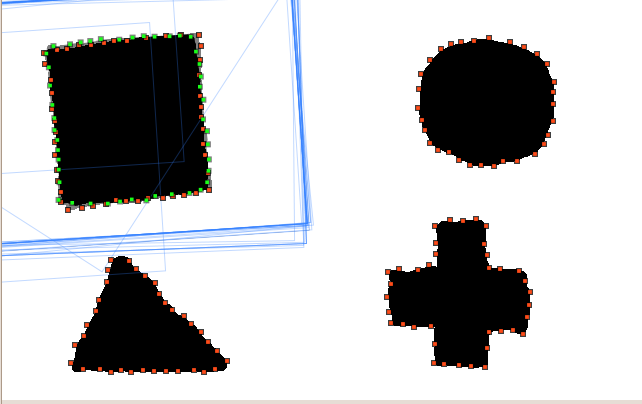
\includegraphics[width=5cm,keepaspectratio=true]{./test1/match1.png}}\hspace{1mm}
\subfloat[krzyż]{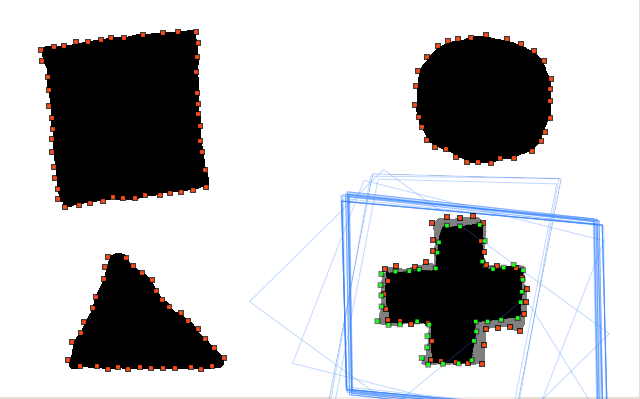
\includegraphics[width=5cm,keepaspectratio=true]{./test1/match2.png}}\hspace{1mm}
\subfloat[koło]{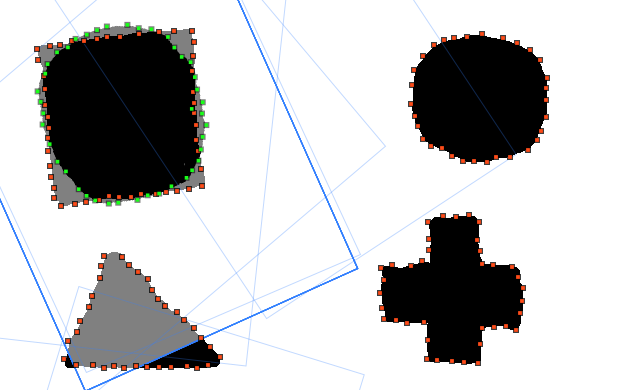
\includegraphics[width=5cm,keepaspectratio=true]{./test1/match3.png}}\hspace{1mm}
\subfloat[trójkąt]{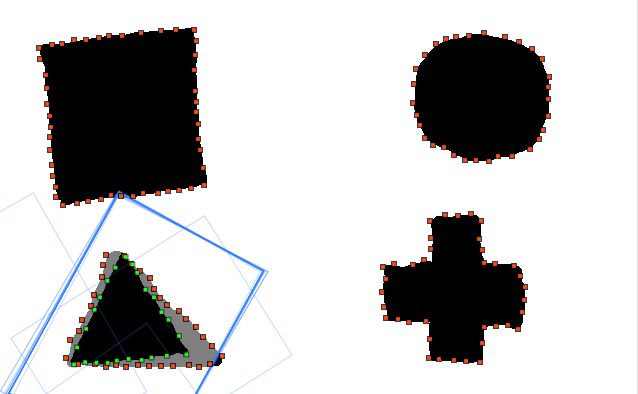
\includegraphics[width=5cm,keepaspectratio=true]{./test1/match4.png}}\hspace{1mm}
\subfloat[gwiazda 5-cio ramienna]{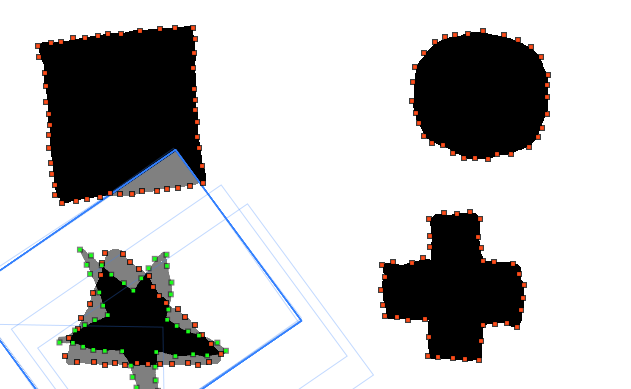
\includegraphics[width=5cm,keepaspectratio=true]{./test1/match5.png}}\hspace{1mm}
\subfloat[gwiazda 4-ro ramienna]{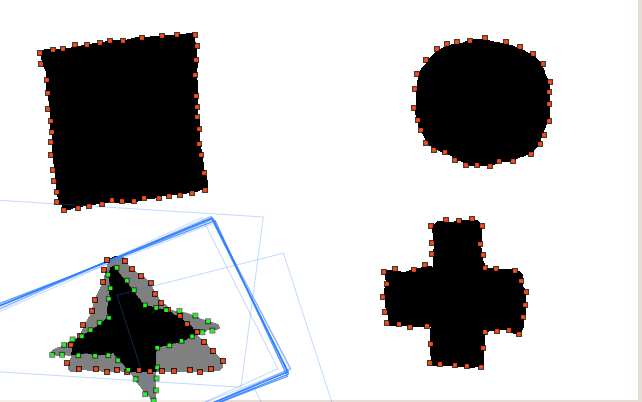
\includegraphics[width=5cm,keepaspectratio=true]{./test1/match6.png}}\hspace{1mm}
\subfloat[dwa koła]{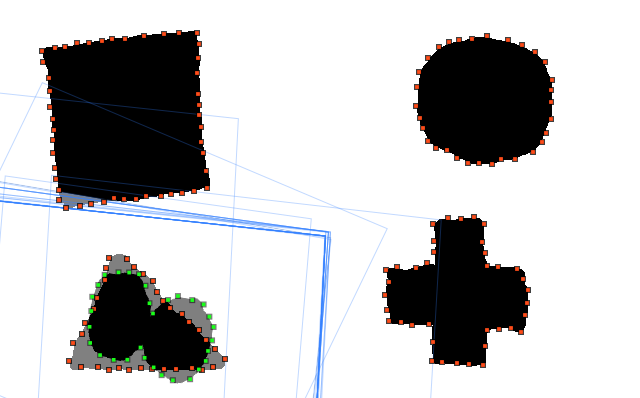
\includegraphics[width=5cm,keepaspectratio=true]{./test1/match7.png}}\hspace{1mm}
\subfloat[podkowa]{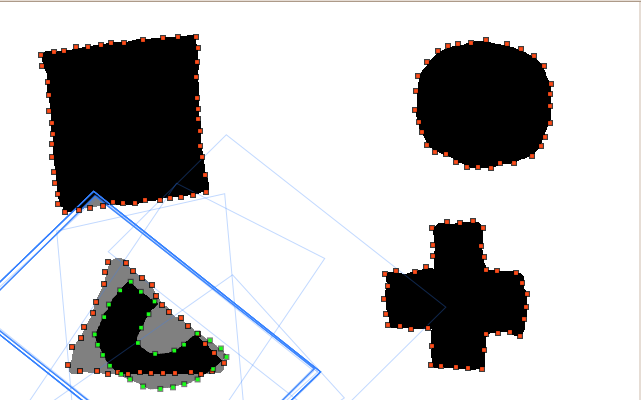
\includegraphics[width=5cm,keepaspectratio=true]{./test1/match8.png}}\hspace{1mm}
\subfloat[4-ro listna koniczyna]{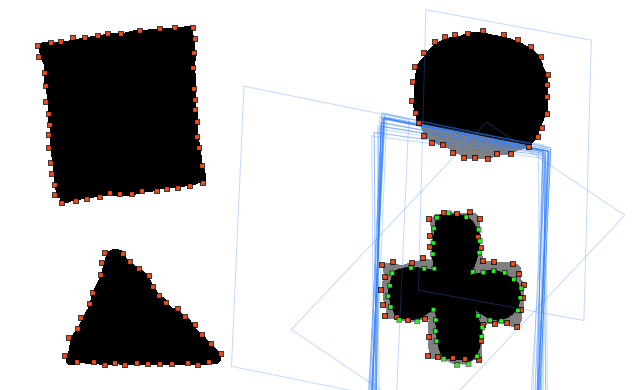
\includegraphics[width=5cm,keepaspectratio=true]{./test1/match9.png}}\hspace{1mm}
\subfloat[domek]{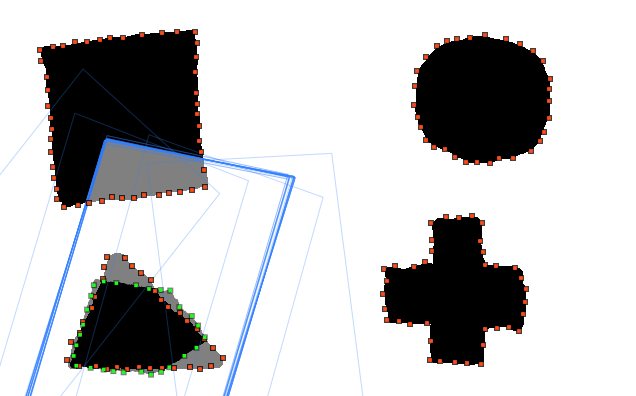
\includegraphics[width=5cm,keepaspectratio=true]{./test1/match10.png}}\hspace{1mm}
\subfloat[screenshot z wyników]{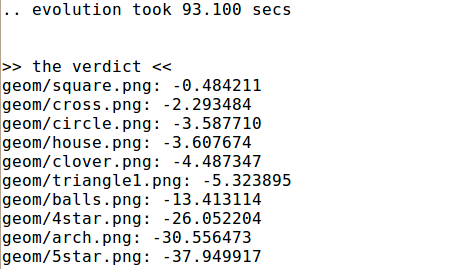
\includegraphics[width=5cm,keepaspectratio=true]{./test1/result.png}}
\caption{Dopasowania figur do mozaiki}{\label{test1-pics}}
\end{figure}

\end{document}
